\documentclass{tufte-book}
%\documentclass[twoside,symmetric]{tufte-book}
\hypersetup{colorlinks}% uncomment this line if you prefer colored hyperlinks (e.g., for onscreen viewing)

%%
% Book metadata

\title{Introduction \\to Python \thanks{Thanks to Edward R.~Tufte for his inspiration.}}
\author[The Tufte-LaTeX Developers]{CSEF}
\publisher{The Student Academy}


%%
% If they're installed, use Bergamo and Chantilly from www.fontsite.com.
% They're clones of Bembo and Gill Sans, respectively.
%\IfFileExists{bergamo.sty}{\usepackage[osf]{bergamo}}{}% Bembo
%\IfFileExists{chantill.sty}{\usepackage{chantill}}{}% Gill Sans

%\usepackage{microtype}

%%
% Just some sample text
\usepackage{lipsum}


%%
% For nicely typeset tabular material
\usepackage{booktabs}

%%
% For graphics / images
\usepackage{graphicx}
\setkeys{Gin}{width=\linewidth,totalheight=\textheight,keepaspectratio}
\graphicspath{{graphics/}}

%%
% Additional
\usepackage{units}
\usepackage{amsmath,amsfonts,amsthm} % Math packages
\usepackage{mathtools}% http://ctan.org/pkg/mathtools
%\usepackage{mparhack}
\usepackage{sectsty} % Allows customizing section commands
\usepackage[dvipsnames]{xcolor}
\usepackage{pgf,tikz}
\usepackage{pgfplots}
\usetikzlibrary{shapes,arrows}
\usetikzlibrary{patterns,fadings}
\usetikzlibrary{arrows}
 \usetikzlibrary{decorations.pathreplacing}
 \usetikzlibrary{snakes}
 \usetikzlibrary{spy}
 \usepackage{setspace}
% \usepackage{3dplot}
 \usepackage{cancel}
%\usepackage{physymb}
\usepackage{braket}
\usepackage{verbatim}
\usepackage{fancyvrb} % extended verbatim environments
\usepackage{framed}%To get shade behind text
\usepackage{pgfplots}
\usepackage{setspace}
\definecolor{shadecolor}{gray}{0.9}
%\usepackage[x11names]{xcolor}                     %Additional colors
%\usepackage{euler}  
\usepackage{framed}

%%%%%%%%%%%%%%%%%%%%%%%%%%%%%%%%%%%%%%%%%%%%%%%%%%%%%
% Default fixed font does not support bold face
\DeclareFixedFont{\ttb}{T1}{txtt}{bx}{n}{12} % for bold
\DeclareFixedFont{\ttm}{T1}{txtt}{m}{n}{12}  % for normal
% Custom colors
\usepackage{color}
\definecolor{normal}{rgb}{0,0.2,1}
\definecolor{lib}{rgb}{0.9,0.5,0}
\definecolor{str}{rgb}{0,0.7,0}
\definecolor{back}{rgb}{0.8,0.8,0.8}

\usepackage{listings}

% Python style for highlighting
\newcommand\pythonstyle{\lstset{
language=Python,
backgroundcolor=\color{back},
basicstyle=\ttm,
otherkeywords={*},             % Add keywords here
keywordstyle=\ttb\color{normal},
emph={__init__, in,from, import, and,not,or,as },          % Custom highlighting
emphstyle=\ttb\color{lib},    % Custom highlighting style
stringstyle=\color{str},
frame=single,
numbers=left,                         % Any extra options here
showstringspaces=false,
stepnumber=1,
commentstyle=\color{red}            % 
}}

% Python environment
\lstnewenvironment{python}[1][]
{
\pythonstyle
\lstset{#1}
}
{}

% Python for external files
\newcommand\pythonexternal[2][]{{
\pythonstyle
\lstinputlisting[#1]{#2}}}

% Python for inline
\newcommand\pythoninline[1]{{\pythonstyle\lstinline!#1!}}


%%%%%%%%%%%%%%%%%%%%%%%%%%%%%%%%%%%%%%%%%%%%%%%%%%%%%%%%%%


% The fancyvrb package lets us customize the formatting of verbatim
% environments.  We use a slightly smaller font.
\usepackage{fancyvrb}
\fvset{fontsize=\normalsize}

%%
% Prints argument within hanging parentheses (i.e., parentheses that take
% up no horizontal space).  Useful in tabular environments.
\newcommand{\hangp}[1]{\makebox[0pt][r]{(}#1\makebox[0pt][l]{)}}

%%
% Prints an asterisk that takes up no horizontal space.
% Useful in tabular environments.
\newcommand{\hangstar}{\makebox[0pt][l]{*}}

%%
% Prints a trailing space in a smart way.
\usepackage{xspace}




% Prints the month name (e.g., January) and the year (e.g., 2008)
\newcommand{\monthyear}{%
  \ifcase\month\or January\or February\or March\or April\or May\or June\or
  July\or August\or September\or October\or November\or
  December\fi\space\number\year
}


% Prints an epigraph and speaker in sans serif, all-caps type.
\newcommand{\openepigraph}[2]{%
  %\sffamily\fontsize{14}{16}\selectfont
  \begin{fullwidth}
  \sffamily\large
  \begin{doublespace}
  \noindent\allcaps{#1}\\% epigraph
  \noindent\allcaps{#2}% author
  \end{doublespace}
  \end{fullwidth}
}

% Inserts a blank page
\newcommand{\blankpage}{\newpage\hbox{}\thispagestyle{empty}\newpage}

\usepackage{units}

% Typesets the font size, leading, and measure in the form of 10/12x26 pc.
\newcommand{\measure}[3]{#1/#2$\times$\unit[#3]{pc}}

% Macros for typesetting the documentation
\newcommand{\hlred}[1]{\textcolor{Maroon}{#1}}% prints in red
\newcommand{\hangleft}[1]{\makebox[0pt][r]{#1}}
\newcommand{\hairsp}{\hspace{1pt}}% hair space
\newcommand{\hquad}{\hskip0.5em\relax}% half quad space
\newcommand{\TODO}{\textcolor{red}{\bf TODO!}\xspace}
\newcommand{\ie}{\textit{i.\hairsp{}e.}\xspace}
\newcommand{\eg}{\textit{e.\hairsp{}g.}\xspace}
\newcommand{\na}{\quad--}% used in tables for N/A cells
\providecommand{\XeLaTeX}{X\lower.5ex\hbox{\kern-0.15em\reflectbox{E}}\kern-0.1em\LaTeX}
\newcommand{\tXeLaTeX}{\XeLaTeX\index{XeLaTeX@\protect\XeLaTeX}}
% \index{\texttt{\textbackslash xyz}@\hangleft{\texttt{\textbackslash}}\texttt{xyz}}
\newcommand{\tuftebs}{\symbol{'134}}% a backslash in tt type in OT1/T1
\newcommand{\doccmdnoindex}[2][]{\texttt{\tuftebs#2}}% command name -- adds backslash automatically (and doesn't add cmd to the index)
\newcommand{\doccmddef}[2][]{%
  \hlred{\texttt{\tuftebs#2}}\label{cmd:#2}%
  \ifthenelse{\isempty{#1}}%
    {% add the command to the index
      \index{#2 command@\protect\hangleft{\texttt{\tuftebs}}\texttt{#2}}% command name
    }%
    {% add the command and package to the index
      \index{#2 command@\protect\hangleft{\texttt{\tuftebs}}\texttt{#2} (\texttt{#1} package)}% command name
      \index{#1 package@\texttt{#1} package}\index{packages!#1@\texttt{#1}}% package name
    }%
}% command name -- adds backslash automatically
\newcommand{\doccmd}[2][]{%
  \texttt{\tuftebs#2}%
  \ifthenelse{\isempty{#1}}%
    {% add the command to the index
      \index{#2 command@\protect\hangleft{\texttt{\tuftebs}}\texttt{#2}}% command name
    }%
    {% add the command and package to the index
      \index{#2 command@\protect\hangleft{\texttt{\tuftebs}}\texttt{#2} (\texttt{#1} package)}% command name
      \index{#1 package@\texttt{#1} package}\index{packages!#1@\texttt{#1}}% package name
    }%
}% command name -- adds backslash automatically
\newcommand{\docopt}[1]{\ensuremath{\langle}\textrm{\textit{#1}}\ensuremath{\rangle}}% optional command argument
\newcommand{\docarg}[1]{\textrm{\textit{#1}}}% (required) command argument
\newenvironment{docspec}{\begin{quotation}\ttfamily\parskip0pt\parindent0pt\ignorespaces}{\end{quotation}}% command specification environment
\newcommand{\docenv}[1]{\texttt{#1}\index{#1 environment@\texttt{#1} environment}\index{environments!#1@\texttt{#1}}}% environment name
\newcommand{\docenvdef}[1]{\hlred{\texttt{#1}}\label{env:#1}\index{#1 environment@\texttt{#1} environment}\index{environments!#1@\texttt{#1}}}% environment name
\newcommand{\docpkg}[1]{\texttt{#1}\index{#1 package@\texttt{#1} package}\index{packages!#1@\texttt{#1}}}% package name
\newcommand{\doccls}[1]{\texttt{#1}}% document class name
\newcommand{\docclsopt}[1]{\texttt{#1}\index{#1 class option@\texttt{#1} class option}\index{class options!#1@\texttt{#1}}}% document class option name
\newcommand{\docclsoptdef}[1]{\hlred{\texttt{#1}}\label{clsopt:#1}\index{#1 class option@\texttt{#1} class option}\index{class options!#1@\texttt{#1}}}% document class option name defined
\newcommand{\docmsg}[2]{\bigskip\begin{fullwidth}\noindent\ttfamily#1\end{fullwidth}\medskip\par\noindent#2}
\newcommand{\docfilehook}[2]{\texttt{#1}\index{file hooks!#2}\index{#1@\texttt{#1}}}
\newcommand{\doccounter}[1]{\texttt{#1}\index{#1 counter@\texttt{#1} counter}}

% Generates the index
\usepackage{makeidx}
\makeindex

\begin{document}

% Front matter
\frontmatter

% r.1 blank page
%\blankpage

% v.2 epigraphs
\newpage\thispagestyle{empty}

\openepigraph{%
The only shibboleth the West has is science. It is the premise of modernity and it defines itself as a rationality capable of, indeed requiring separation from politics, religion and really, society. Modernisation is to work towards this.
}{Bruno Latour}
\vfill
\openepigraph{%
The boundary between science fiction and social reality is an optical illusion.
}{Donna Haraway}


% r.3 full title page
\maketitle




% r.5 contents
\tableofcontents

\listoffigures

\listoftables

% r.7 dedication
\cleardoublepage
~\vfill
\begin{doublespace}
\noindent\fontsize{18}{22}\selectfont\itshape
\nohyphenation
The longest snake ever held captive is Medusa, a reticulated python (python reticulatus). On 12 October 2011, she was measured at 7.67 m long.% \mbox{Edward R.~Tufte} 
%and \mbox{Donald E.~Knuth}.
\end{doublespace}
\vfill
\vfill


% r.9 introduction
%\cleardoublepage
\chapter*{Note}

This physics text is an OpenSource academic project developed in abstraction at The Academy.  The manuscript is written in \LaTeX \ and makes use of the \doccls{tufte-book} and \doccls{tufte-handout} document classes.  

\vspace{2cm}

http://latex-project.org/ftp.html

https://git-scm.com/downloads

%%
% Start the main matter (normal chapters)
\mainmatter


\include{Terminal}
\include{git}
\include{latex}
\include{array}
\include{int_and_floatz}
\include{booleans_michael}
\include{while_loops}
\include{while}
\include{Bases}
\include{array}
\include{Arrays}
\include{for_loop}
\include{libraries_intro}
\include{random}
\include{Statistics}
\include{stats17}
\include{Libraries_Graphics}
\include{Monte_Carlo}
\include{Game_of_Life}
\chapter{Latex}
LaTeX is a document preparation system for high-quality typesetting. It is most often used for medium-to-large technical or scientific documents but it can be used for almost any form of publishing. 

\marginnote
\begin{figure}	
    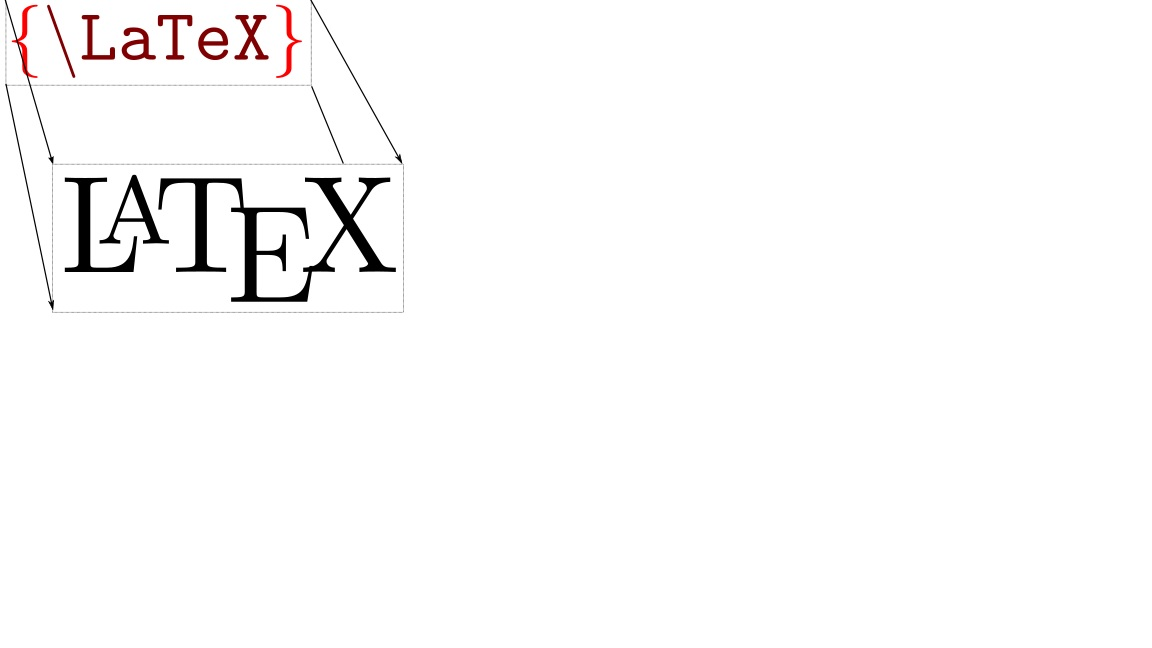
\includegraphics[width=10cm]{1}
\end{figure}

\section{Using of the latex}

The Latex is used for writing the essay such as about Codes, mathmatic functions, graphics etc. This tool is useful as you try to put images into your assignment, because there are a lot of ways to do it. Actually not only putting images but also differentiating the section of your part. 

\begin{figure}
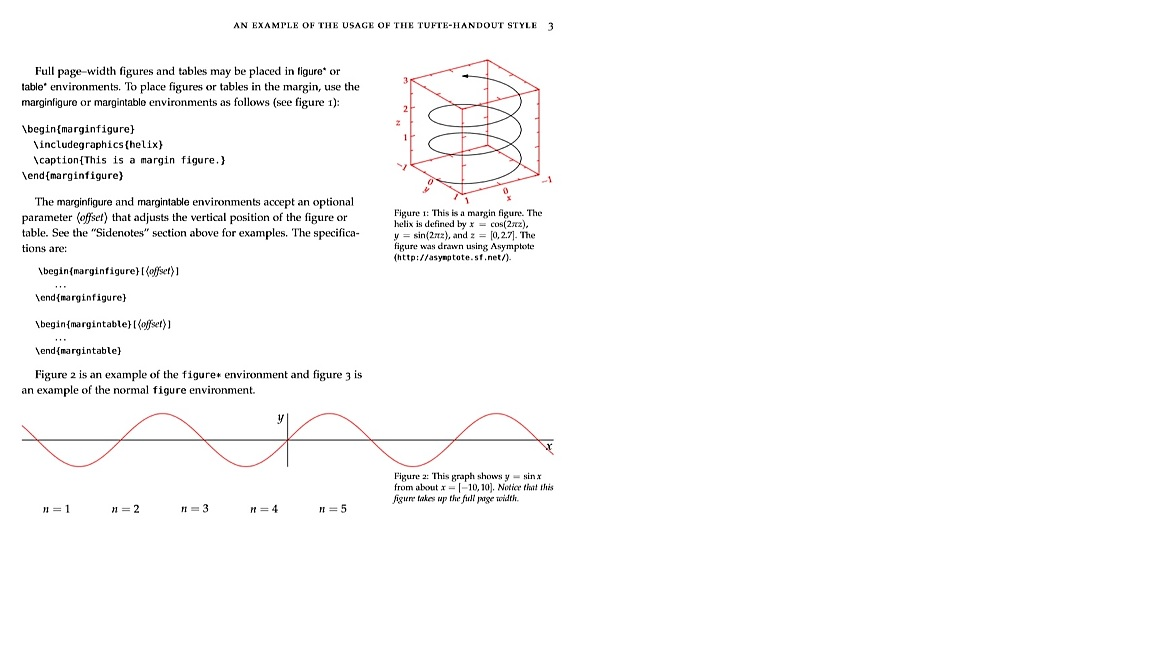
\includegraphics[width=10cm]{123}
\end{figure}

\section{The features of using Latex}
A.Typesetting journal articles, technical reports, books, and slide presentations.
B.Control over large documents containing sectioning, cross-references, tables and figures.
C.Typesetting of complex mathematical formulas.
D.Advanced typesetting of mathematics with AMS-LaTeX.
E.Automatic generation of bibliographies and indexes.
F.Multi-lingual typesetting.
G.Inclusion of artwork, and process or spot colour.
H.Using PostScript or Metafont fonts.

\begin{figure}
	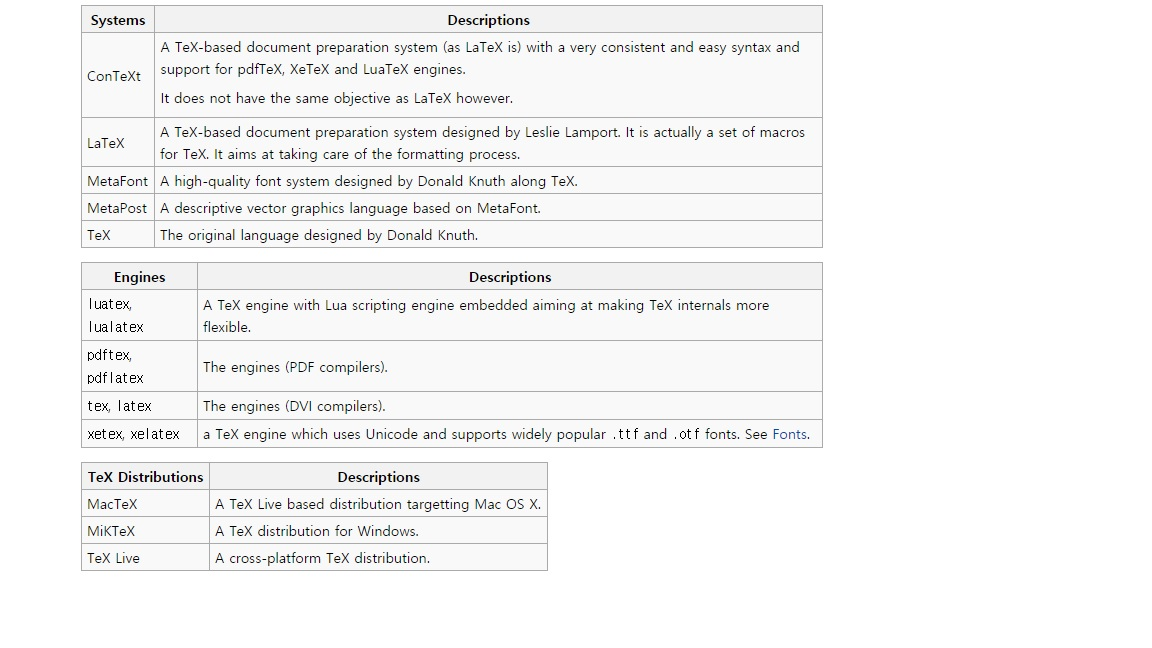
\includegraphics[width=10cm]{234}
\end{figure}

Latex is also easy to use for beginner There are a lot of tools to begin writing essaies. When beginner doesn't know how to use, they would be able to search the solutions from the internet web sites. 
	






%\bibliography{sample-handout}
\bibliographystyle{plainnat}



\printindex

\end{document}


